% ncse_new/\problems/ch_piecewisepolynomials/ex_GradedMeshes.tex
% exercise requires:   GradedMesh.eps
% solutions require:   PWlineConv.m  PWlineIntp.m  PWlineConv.eps  GradedMesh.m  PWlineGraded.m  PWlineGraded_0.50.eps

\begin{problem}[Piecewise linear approximation on graded meshes \coreproblem]
  \label{prb:GradedMeshes}

One of the messages given by \lref{sec:ChebychevInterpolation}
is that the quality of an interpolant depends heavily on the choice of the
interpolation nodes.  If the function to be interpolated has a ``bad behavior'' in
a small part of the domain, for instance it has very large derivatives of high
order, more interpolation points are required in that area of the domain.
Commonly used tools to cope with this task, are \textit{graded meshes}, which
will be the topic of this problem.

\vspace{4mm}

Given a mesh $\Ct=\{0\le t_0<t_1<\cdots<t_n\le1\}$ on the unit interval $I=[0,1]$, $n\in\IN$, we define the \textit{piecewise linear} interpolant
$$\Isf_\Ct:C^0(I)\rightarrow \Cp_{1,\Ct} = \{ s\in C^0(I),\; s_{|[t_{j-1},t_j]}\in\Cp_1\;\forall\;j \},
\quad\text{s.t.}\quad \big(\Isf_\Ct f\big) (t_j)=f(t_j),\quad j=0,\ldots,n; $$
(see also \lref{sec:piecewise-linear-interp}).


\begin{subproblem}[2]
\label{subprb:GradedMeshes_1}
If we choose the uniform mesh $\Ct=\{t_j\}_{j=0}^n$ with $t_j=j/n$, given a function $f\in C^2(I)$, what is the asymptotic behavior of the error
$$\N{f-\Isf_\Ct f}_{L^\infty(I)},$$
when $n\rightarrow\infty$?

\begin{hint}
Look for a suitable estimate in \lref{sec:ppi}.
\end{hint}

\begin{solution}
Equation \ncseeq{pwintp:LinfConv} says
$$\N{f-\Isf_\Ct f}_{L^\infty(I)}  \leq \frac1{2n^2}\N{f^{(2)}}_{L^\infty(I)}, $$
because the meshwidth is $h=1/n$. So, the convergence is quadratic, i.e., algebraic with order 2.
\end{solution}
\end{subproblem}



%%%%%%%%%%%%%%%%%%%%%%%%%%%%%%%%%%%%%%%%%%%%%%%%%%%%%%%%%%%

\begin{subproblem}[2]\label{subprb:GradedMeshes_2}
What is the regularity of the function
$$f:I\rightarrow\IR,\qquad f(t)=t^\alpha, \qquad 0<\alpha<2\;?$$
In other words, for which $k\in\IN$ do we have $f\in C^k(I)$? 

\begin{hint}
Notice that $I$ is a closed interval and check the continuity of the derivatives in the endpoints of $I$.
\end{hint}

\begin{solution}
If $\alpha=1$, $f(t)=t$ clearly belongs to $C^\infty(I)$.
If $0<\alpha<1$, $f'(t)=\alpha t^{\alpha-1}$ blows up to infinity for $t$ going to $0$, therefore $f\in C^0(I)\setminus C^1(I)$.
If $1<\alpha<2$, $f'$ is continuous but $f''(t)=\alpha(\alpha-1) t^{\alpha-2}$ blows up to infinity for $t$ going to $0$, 
therefore $f\in C^1(I)\setminus C^2(I)$.

More generally, for $\alpha\in \IN$ we have $f(t)=t^\alpha\in C^\infty(I)$; on the other hand if $\alpha>0$ is not an integer, $f\in C^{\lfloor \alpha\rfloor}(I)$, where $\lfloor \alpha\rfloor =\mathrm{floor}(\alpha) $ is the largest integer not larger than $\alpha$.
\end{solution}
\end{subproblem}





%%%%%%%%%%%%%%%%%%%%%%%%%%%%%%%%%%%%%%%%%%%%%%%%%%%%%%%%%%%

\begin{subproblem}[3]\label{subprb:GradedMeshes_2half}
Study numerically the $h$-convergence of the piecewise linear approximation of
$f(t)=t^\alpha$ ($0<\alpha<2$) on uniform meshes; determine the order of
convergence using linear regression based on \Matlab's \texttt{polyfit}, see
\ncsesect{sec:ppi}.

\begin{hint}
Linear regression and \texttt{polyfit} have not been introduced yet. Please give a quick look at the examples in \href{http://ch.mathworks.com/help/matlab/ref/polyfit.html\#examples}{http://ch.mathworks.com/help/matlab/ref/polyfit.html\#examples} to see \texttt{polyfit} in action. For instance, the code to determine the slope of a line approximating a sequence of points $(x_i,y_i)_i$ in doubly logarithmic scale is
\begin{lstlisting}
P = polyfit(log(x),log(y),1);
slope = P(1);
\end{lstlisting}
\end{hint}

\begin{solution}The interpolant is implemented in Listing~\ref{mc:PWlineIntp}, the convergence for our choice of $f$ is studied in file \texttt{PWlineConv.m} and the results are plotted in Figure~\ref{fig:PWlineConv}.
The convergence is clearly algebraic, the rate is equal to $\alpha$ if it is smaller than 2, and equal to 2 otherwise.
In  brief, we can say that the order is $\min\{\alpha,2\}$.

Be careful with the case $\alpha=1$: here the interpolant gets exactly the solution, with every mesh.

\lstinputlisting[caption={Piecewise linear interpolation.},label={mc:PWlineIntp}]
{\problems/ch_piecewisepolynomials/MATLAB/PWlineIntp.m}


\begin{figure}[htb]
\caption{$h$-convergence of piecewise linear interpolation for $f(t)= t^\alpha$, $\alpha=0.1,0.3,\ldots,2.9$.
The convergence rates are shown in the small plot.}
\label{fig:PWlineConv}\begin{center}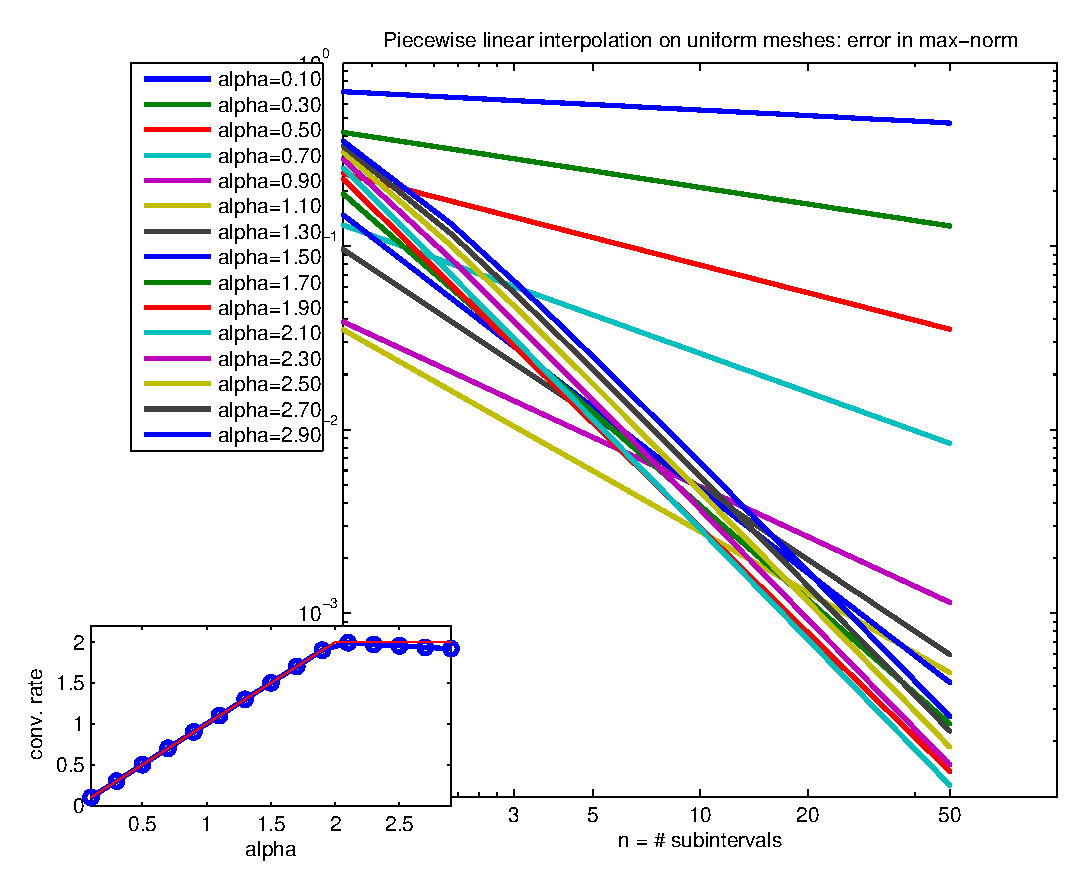
\includegraphics[width=0.85\textwidth]{\problems/ch_piecewisepolynomials/PICTURES/PWlineConv.eps}\end{center}\end{figure}
\end{solution}
\end{subproblem}





%%%%%%%%%%%%%%%%%%%%%%%%%%%%%%%%%%%%%%%%%%%%%%%%%%%%%%%%%%%

\begin{subproblem}[3]\label{subprb:GradedMeshes_3}
In which mesh interval do you expect $|f-\Isf_{\Ct}f|$ to attain its maximum?

\begin{hint}
You may use the code from the previous subtask to get an idea.
\end{hint}
\begin{hint}
What is the meaning of \ncsethm{cor:polintperr}  in the piecewise linear setting? 
\end{hint}

\begin{solution}The error representation \ncseeq{intp:thm-error-estim} in the linear case ($n=1$) reads
\begin{align*}
 \forall\;t\in(t_j,t_{j+1})\qquad  \Big|f(t)-\big(\Isf_{\Ct}f\big)(t)\Big| &=\frac12 |f''(\tau_t) \; (t-t_j)(t-t_{j+1})| \\
&\leq \frac18 |f''(\tau_t)|\; (t_{j+1}-t_{j})^2 = \frac1{8n^2}|f''(\tau_t)|,
\end{align*}
for some $\tau_t\in(t_j,t_{j+1})$.
Therefore the error can be large only in the subintervals where the second derivative of $f$ is large.
But
$$|f''(t)|=\big|\alpha(\alpha-1)t^{\alpha-2}\big|$$
is monotonically decreasing for $0<\alpha<2$, therefore we can expect a large error in the first subinterval, the one that is closer to $0$.

In line 23 of the code in \texttt{PWlineConv.m},  we check our guess: the maximal error is found in the first interval for every $\alpha\in(0,2)$ ($\alpha\ne1$) and in the last one for $\alpha>2$.
\end{solution}
\end{subproblem}




%%%%%%%%%%%%%%%%%%%%%%%%%%%%%%%%%%%%%%%%%%%%%%%%%%%%%%%%%%%

\begin{subproblem}[3]\label{subprb:GradedMeshes_4}
Compute by hand the exact value of $\N{f-\Isf_{\Ct}f}_{L^\infty(I)}$.

Compare the order of convergence obtained with the one observed numerically in \ref{subprb:GradedMeshes_2}.

\begin{hint}
Use the result of \ref{subprb:GradedMeshes_3} to simplify the problem.
\end{hint}

\begin{solution}From \ref{subprb:GradedMeshes_3} we expect that the maximum is taken in the first subinterval.
For every  $t\in(0,1/n)$ and $0<\alpha<2$ ($\alpha\ne1$) we compute the minimum of the error function $\varphi$ 
\begin{align*}
\varphi(t)   &=f(t)-\big(\Isf_{\Ct}f\big)(t) = t^\alpha- t\;\frac1{n^{\alpha-1}},\hspace{2cm}(\varphi(0)=\varphi(1/n)=0),\\
\varphi'(t)  &= \alpha t^{\alpha-1}- \frac1{n^{\alpha-1}},\\
\varphi'(t^*)&=0\quad\text{if}\quad t^* = \frac 1n\alpha^{1/(1-\alpha)} \le\frac1{2n},\\          % <=1/2   is not easy.....
\max_{t\in(0,1/n)}|\varphi(t)|&=|\varphi(t^*)|=\Big|\frac{\alpha^{\alpha/(1-\alpha)}}{n^\alpha}-\frac{\alpha^{1/(1-\alpha)}}{n^\alpha}\Big|
              =\frac1{n^\alpha}\Big|\alpha^{\alpha/(1-\alpha)}-\alpha^{1/(1-\alpha)}\Big|    = \Co(n^{-\alpha}) = \Co(h^{\alpha}).
\end{align*}
The order of convergence in $h=1/n$ is equal to the parameter $\alpha$, as observed in Figure~\ref{fig:PWlineConv}.
\end{solution}
\end{subproblem}



%%%%%%%%%%%%%%%%%%%%%%%%%%%%%%%%%%%%%%%%%%%%%%%%%%%%%%%%%%%

\begin{subproblem}[3]\label{subprb:GradedMeshes_5}
Since the interpolation error is concentrated in the left part of the domain, it seems reasonable to use a finer mesh only in this part.
A common choice is an \textbf{algebraically graded mesh}, defined as
$$\Cg=\Big\{t_j=\Big(\frac jn\Big)^\beta,\quad j=0,\ldots,n\Big\},$$
for a parameter $\beta>1$.
An example is depicted in Figure~\ref{fig:GradedMesh} for $\beta=2$.

\begin{figure}[htb]\caption{Graded mesh $x_j=(j/n)^2$, $j=0,\ldots,10$.}\label{fig:GradedMesh}
\begin{center}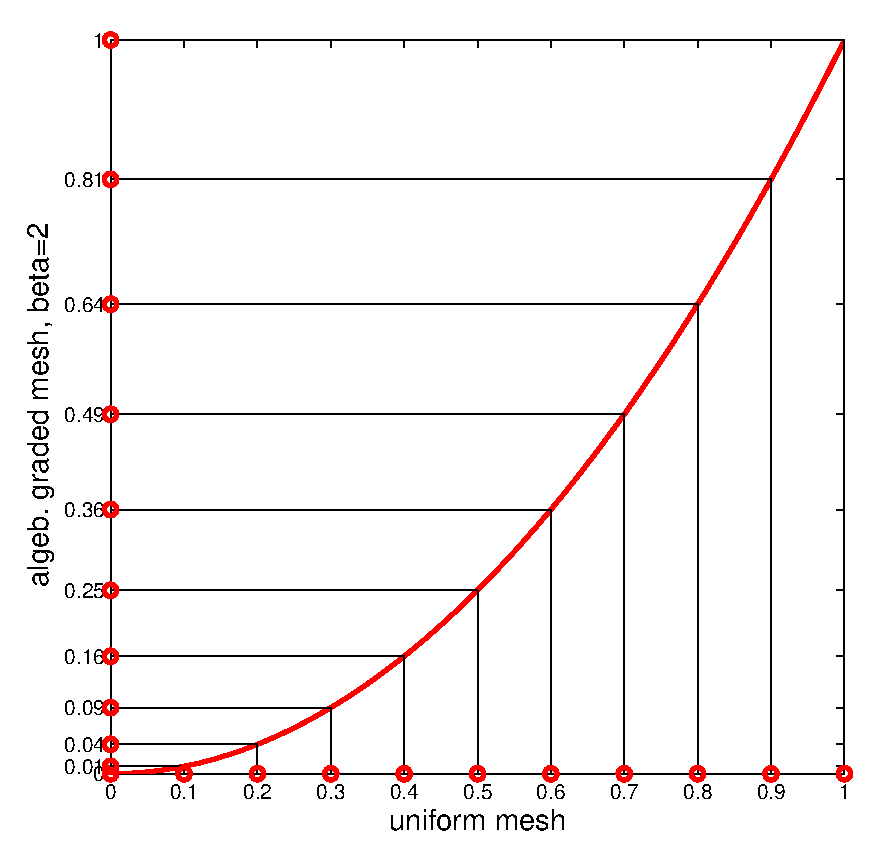
\includegraphics[width=0.5\textwidth]{\problems/ch_piecewisepolynomials/PICTURES/GradedMesh.eps}\end{center}\end{figure}

For a fixed parameter $\alpha$ in the definition of $f$, numerically determine the rate of convergence of the piecewise linear interpolant $\Isf_\Cg$ on the graded mesh $\Cg$ as a function of the parameter $\beta$.
Try for instance $\alpha=1/2$, $\alpha=3/4$ or $\alpha=4/3$.

How do you have to choose $\beta$ in order to recover the optimal rate $\Co(n^{-2})$ (if possible)?  


\begin{solution}The code in file \texttt{PWlineGraded.m} studies the dependence of the convergence rates on $\beta$ and $\alpha$.
The result for $\alpha=0.5$ is plotted in Figure~\ref{fig:PWlineGraded}.

The comparison of this plot with the analogous ones for different values of $\alpha$ suggests that the choice of $\beta=2/\alpha$ guarantees quadratic convergence, run the code to observe it.

Proceeding as in \ref{subprb:GradedMeshes_4}, we can see that the maximal error in the first subinterval $(0,t_1)=(0,1/n^\beta)$ is equal to
$1/n^{\alpha\beta} \;(\alpha^{\alpha/(1-\alpha)}-\alpha^{1/(1-\alpha)})=\Co(n^{-\alpha\beta})$.
This implies that a necessary condition to have quadratic convergence is $\beta\geq 2/\alpha$.
In order to prove un upper bound on the optimal $\beta$, we should control the error committed in every subinterval, here the exact computation of $\varphi(t^*)$ becomes quite long and complicate.

For larger values of the grading parameter, the error in last few subintervals begins to increase.
The variable \texttt{LocErr} contains the index of the interval where the maximal error is attained (take a look at its values).
It confirms that the largest error appears in the first subinterval if $\alpha\beta\ll 2$ and in the last one if $\alpha\beta\gg2$, the intermediate cases are not completely clear.


\begin{figure}[htb]
\caption{$h$-convergence of piecewise linear interpolation for $f(t)= t^\alpha$, $\alpha=0.5$, on algebraically graded meshes with parameters $\beta\in[1,5]$.
The convergence rates in dependence on $\beta$ are shown in the small plot.}
\label{fig:PWlineGraded}\begin{center}\includegraphics[width=0.85\textwidth]{\problems/ch_piecewisepolynomials/PICTURES/PWlineGraded_050.eps}\end{center}\end{figure}

Figure~\ref{fig:GradedMesh} has been created with the code in Listing~\ref{mc:GradedMesh}.
\lstinputlisting[caption={Plot of algebraically graded mesh.},label={mc:GradedMesh},escapechar={}]
{\problems/ch_piecewisepolynomials/MATLAB/GradedMesh.m}
\end{solution}
\end{subproblem}

\end{problem}

%